\def \tyPlain {Implementation in Plain Xtext}
\def \tyPlusPlain {The Plus Operator in Plain Xtext}
\section[Plain Xtext]{\tyPlain}

\begin{frame}
  \tableofcontents[currentsection]
\end{frame}

\begin{frame}[fragile]
  \frametitle{\tyPlain}
  \begin{itemize}
    \item Implementation in Xtend
    \begin{itemize}
      \item Type provider - recursive computation
      \item Type conformance computer
      \item Xtext validator hook
    \end{itemize}
  \end{itemize}
\end{frame}

%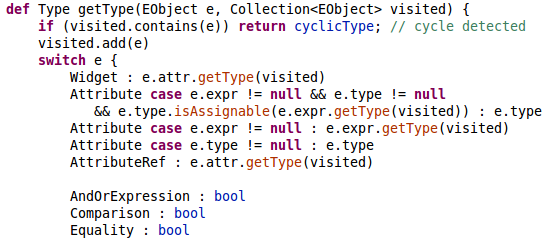
\includegraphics[width=.9\textwidth]{img/plain-xtext-provider.png}

\begin{frame}[fragile]
  \frametitle{\tyPlusPlain}
  \begin{itemize}
    \item Type Provider 
  \end{itemize}

  \begin{footnotesize}
    % Generator: GNU source-highlight, by Lorenzo Bettini, http://www.gnu.org/software/src-highlite
\begin{tabular}[t]{l}
\noindent
\mbox{}\textbf{\textcolor{Plum}{def}}\ Type\ \textcolor{Black}{getExpectedType}(EObject\ e)\ \{ \\
\mbox{}\ \ \ \ ... \\
\mbox{}\ \ \ \ \textbf{\textcolor{Plum}{switch}}\ e\ \{ \\
\mbox{}\ \ \ \ \ \ \ \ ... \\
\mbox{}\ \ \ \ \ \ \ \ Plus\ :\ \ \textcolor{Black}{mostGeneral}(e.left.type,\ e.right.type).\textcolor{Black}{mostSpecific}(string)\ \ \ \ \  \\
\mbox{} \\
\mbox{}\textbf{\textcolor{Plum}{def}}\ Type\ \textcolor{Black}{mostGeneral}(Type\ one,\ Type\ two)\ \{ \\
\mbox{}\ \ \ \ \textbf{\textcolor{Plum}{if}}\ (\textcolor{Black}{isAssignable}(one,\ two)) \\
\mbox{}\ \ \ \ \ \ one\  \\
\mbox{}\ \ \ \ \ \ \ \ \textbf{\textcolor{Plum}{else}} \\
\mbox{}\ \ \ \ \ \ two \\
\mbox{}\ \ \ \ \} \\
\mbox{} \\
\mbox{}\textcolor{Green}{//\ allow\ numbers\ where\ strings\ are\ expected} \\
\mbox{}\textbf{\textcolor{Plum}{def}}\ \textbf{\textcolor{Plum}{dispatch}}\ \textcolor{Black}{isAssignable}(StringType\ left,\ NumberType\ right)\ \{\ \textbf{\textcolor{Plum}{true}}\ \} \\
\mbox{}\ \ \ \ \ \ \ \ 
\end{tabular}

  \end{footnotesize}
\end{frame}

\begin{frame}[fragile]
  \frametitle{\tyPlusPlain}
  \begin{itemize}
    \item Type Conformance 
  \end{itemize}

  \begin{footnotesize}
    % Generator: GNU source-highlight, by Lorenzo Bettini, http://www.gnu.org/software/src-highlite
\begin{tabular}[t]{l}
\noindent
\mbox{}...\  \\
\mbox{}\textbf{\textcolor{Plum}{def}}\ \textbf{\textcolor{Plum}{dispatch}}\ \textcolor{Black}{isAssignable}(Type\ left,\ Type\ right)\ \{\ ...\ \} \\
\mbox{}... \\
\mbox{}\textbf{\textcolor{Plum}{def}}\ \textbf{\textcolor{Plum}{dispatch}}\ \textcolor{Black}{isAssignable}(StringType\ left,\ NumberType\ right)\ \{\ \textbf{\textcolor{Plum}{true}}\ \} \\
\mbox{}...
\end{tabular}

  \end{footnotesize}
\note{
  def Type mostGeneral(Type one, Type two) {
	if (isAssignable(one, two))
	  one 
	    else
	  two
	} \\
  // allow numbers where strings are expected
}
\end{frame}